%%%% PLEASE REPLACE ENTIRELY WITH YOUR OWN CONTENT %%%%

\chapter{Introduction}
In recent years, we have witnessed a technological revolution. Devices have evolved at an extraordinary pace, reaching a level of sophistication that has brought computing to a point where improving the hardware of traditional devices presents significant challenges.

This improvement has been achieved, in part, through the reduction in the size of transistors, a principle described by Dennard Scaling in 1974. This principle indicates that by reducing the size of transistors, both their performance and efficiency are improved. Additionally, an important empirical observation is Moore's Law, which states that the number of transistors in a microprocessor doubles every two years.

These two phenomena have led to exponential growth in processing capacity.Nevertheless,physical and technological limitations have halted the ability to further reduce the size of transistors. For this reason, research into alternatives to classical computing has become one of the main objectives for many companies today.

It has been observed that quantum computing is particularly effective in certain fields, one of which is quantum simulation. In this project, we will use quantum computing to simulate molecular systems, focusing on achieving efficient and precise quantum simulations. To this end, advanced methodologies have been implemented to improve efficiency and resource utilization on a classical computer, and the Variational Quantum Eigensolver (VQE) algorithm has been employed, which will be explained in greater detail later.

\section{Work goals}
The main objective of our project has been to develop a method to parallelize evaluations of quantum molecular dynamics simulations. To this end, the following objectives have been declared:

\begin{itemize}
  \item Optimize the quantum simulation framework to minimize computational overhead while maintaining accuracy in modeling molecular systems.
  \item Integrate an adaptive quantum ansatz capable of dynamically selecting and integrating operators with the highest impact on performance, ensuring rapid convergence and reduced computational cost.
  \item Integrate advanced hybrid optimization cycles that streamline both electronic state and nuclear geometry refinements, with an emphasis on computational speed and scalability.
  \item Design a high-performance, modular architecture tailored for extensibility, facilitating the efficient inclusion of ansatz designs, optimization strategies and different types of molecules.
\end{itemize}


\section{Requirements and specifications}

To achieve these objectives, the following requirements and specifications have been established:

\begin{itemize}
  \item \textbf{Dynamic Quantum Circuit Construction}: Integrate an adaptive quantum circuit mechanism that employs energy gradient calculations to iteratively select and include the most impactful operators, reducing the complexity of the quantum circuits without compromising accuracy.
  \item \textbf{Advanced Hybrid Optimization}: Develop a unified optimization cycle combining variational parameter updates and nuclear geometry refinements, supported by precise gradient-based techniques. Ensure the use of optimizers for rapid convergence and enhanced stability.
  \item \textbf{Scalable System Representation}: Implement a modular system construction process that accommodates different molecular geometries and basis sets with efficient computation of molecular properties.
  \item \textbf{Efficient Gradient Computation}: Optimize gradient calculations for both quantum and nuclear coordinates using automatic differentiation, enabling simultaneous updates and faster convergence.
  \item \textbf{Performance Monitoring and Visualization}: Develop tools for tracking energy convergence, execution time, and molecular geometry evolution. Include detailed visualizations (e.g., energy evolution plots, 3D geometries) to ensure transparency and allow performance analysis.
  \item \textbf{Extensibility and Modularity}: Ensure a modular project structure that facilitates the inclusion of new ansatz types, optimizers, and molecular systems with minimal adjustments. Employ a structured directory for clear separation of functionality and scalability.
  \item \textbf{Parallel Execution Capability}: Leverage multiprocessing capabilities to evaluate multiple optimizers and configurations in parallel, enabling comprehensive performance analysis across various configurations.
\end{itemize}


\section{Methods and procedures}
To achieve the objectives of this project, we carried out a series of implementations to achieve the previously mentioned objectives. As an initial phase, the existing frameworks currently on the market were compared to begin the development of our project. Next, a first, basic version was developed to simulate a single molecule with a single configuration.

In the first version of the project, a single quantum simulation was developed with the aim of verifying that the framework worked correctly and allowed us to use it for our project. Once this was verified, the next step was to begin developing the modular structure of the project, which would facilitate the integration of new components into our project. This modular structure would allow us to compare the different components of our quantum molecular dynamics simulator.

Subsequently, a series of techniques were implemented, integrating quantum classical algorithms, to find the lowest energy values in our simulations. Additionally, the integration of the modular structure facilitated the implementation of configurations for our simulations, allowing us to make different configurations and thus find these minimum values more efficiently.

By modularizing the project, it became possible to parallelize different simulation configurations, as by modifying the variable values, we could simulate different molecules and internal configurations of the optimizer.

Finally, tools were implemented to visualize the results and store them automatically and easily. These results are especially important as they allow us to analyze the obtained data in greater depth, enabling us to draw more precise conclusions.

\section{Work plan}

During the development of the project, the initial plan was largely followed. However, several complications arose that extended some deadlines, requiring adjustments to the overall timeline to achieve the established objectives.

The main setback was related to the integration of the JAX interface. From the outset, we were confident that using JAX would significantly improve the performance of the simulations. However, upon completing the initial integration, we were surprised to find that the performance not only failed to improve but actually worsened. This unexpected result led us to conduct more checks than initially planned, aiming to verify the accuracy of the results and identify the root cause of this behavior.

This situation caused delays in the second phase of the project, which, in turn, required a reduction in the time allocated to the third phase to meet the deadlines. Despite this, we decided not to compromise on the quality of the project. As a result, the overall development time had to be extended, increasing the daily hours dedicated to the project. This additional effort ensured that the initial objectives were achieved without compromising the proposed quality standards.

\begin{figure}[H]
  \centering
  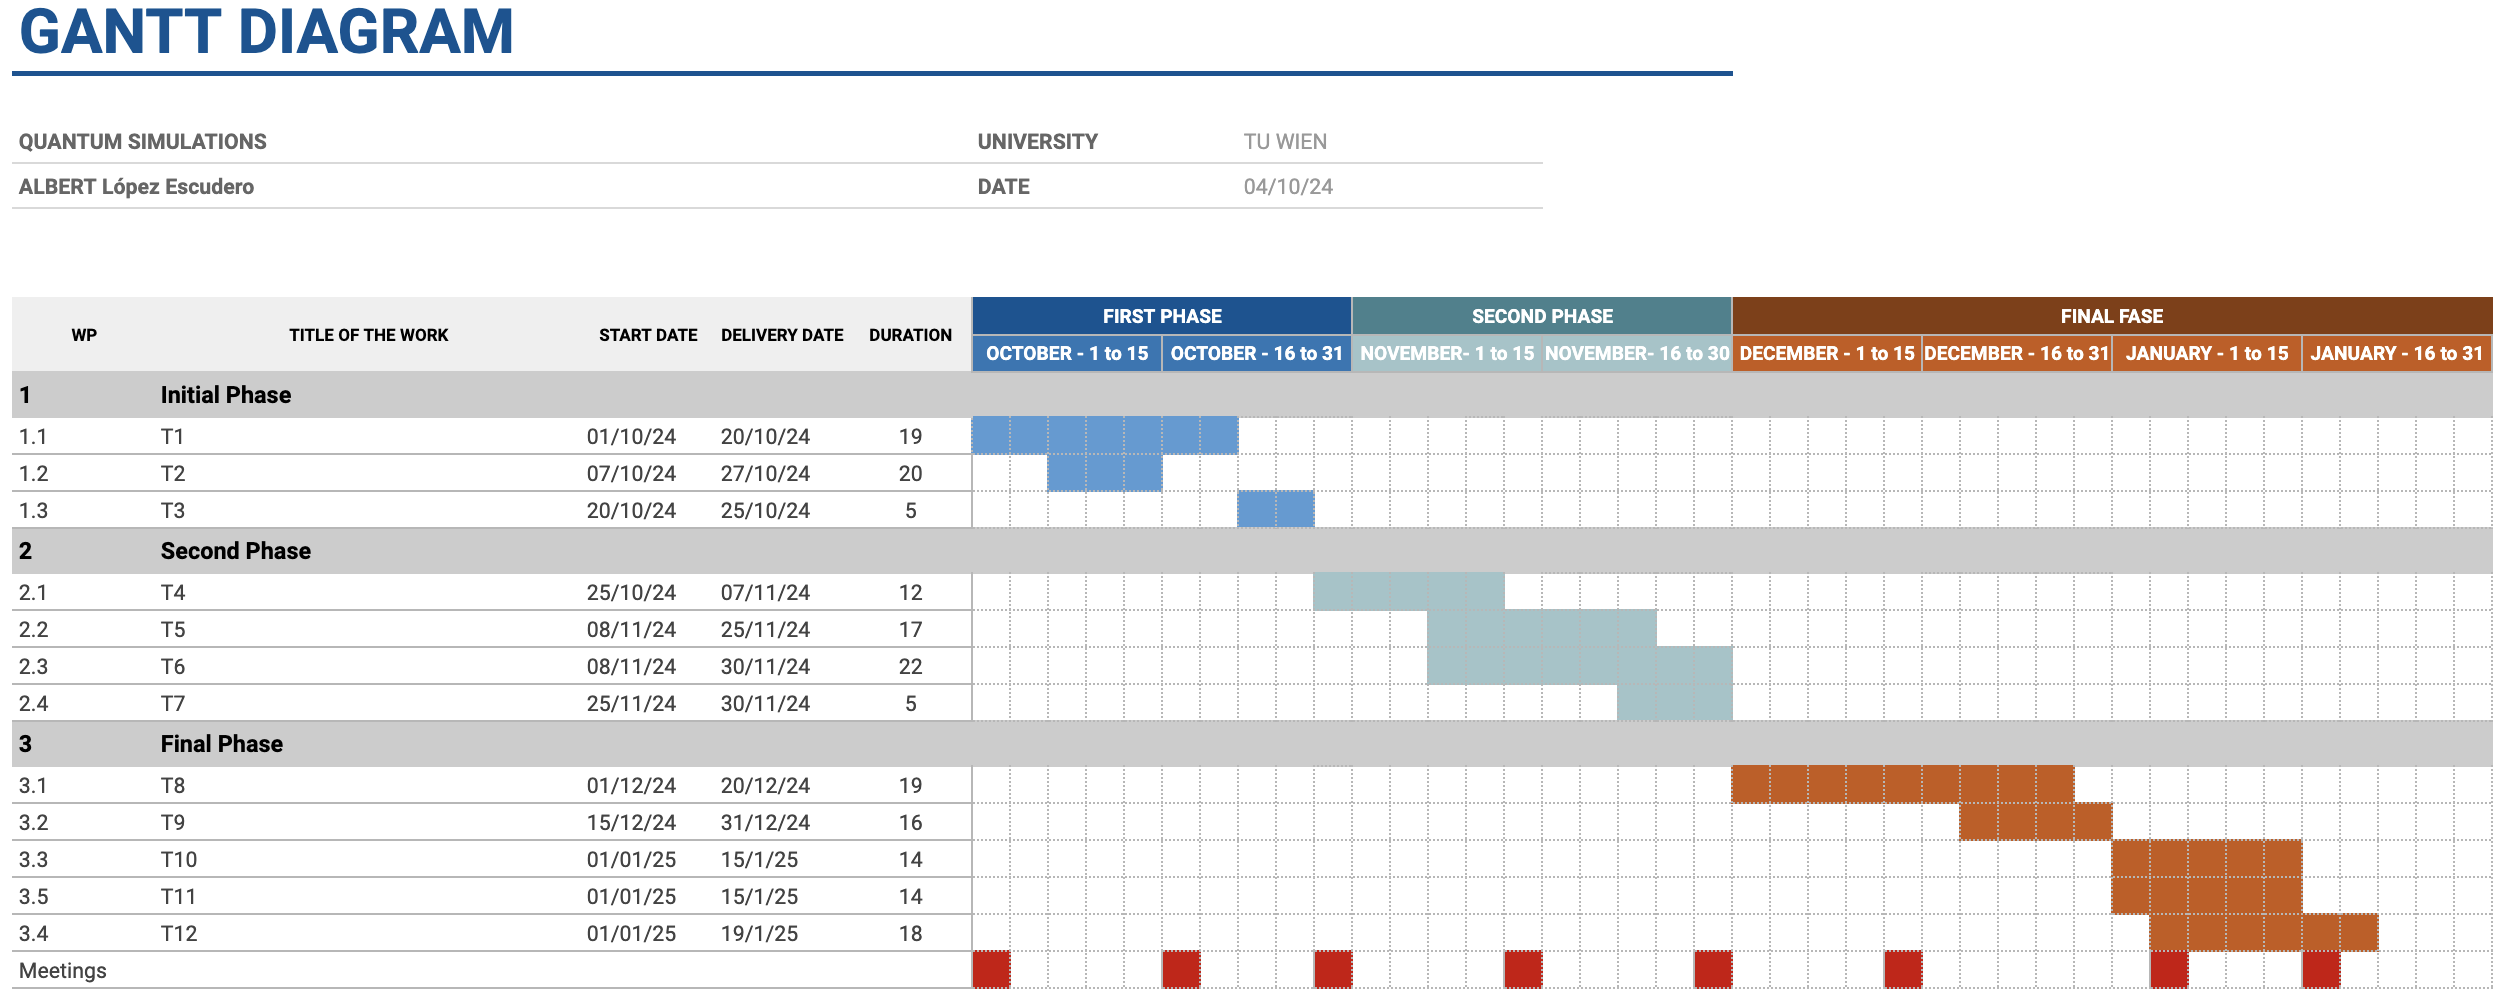
\includegraphics[width=1\textwidth]{img/Gantt_diagram.png}
  \caption{Gantt diagram showing the project timeline and the distribution of tasks over the development period.}
  \label{fig:gantt_diagram}
\end{figure}